\subsubsection{Giới thiệu bộ dữ liệu}
    \paragraph{Nguồn dữ liệu}
    \leavevmode

    Bộ dữ liệu là bộ dữ liệu hình ảnh do tác giả Ahmed Saied thu thập cho cuộc thi NASA Space Apps.

    \paragraph{Mô tả dữ liệu}
    \leavevmode

    Bộ dữ liệu chứa các hình ảnh có hoặc không có lửa cháy trong hình. Dữ liệu có 999 hình ảnh tổng cộng.

    Ví dụ một phần dữ liệu:

    \begin{figure}[htp]
        \centering
        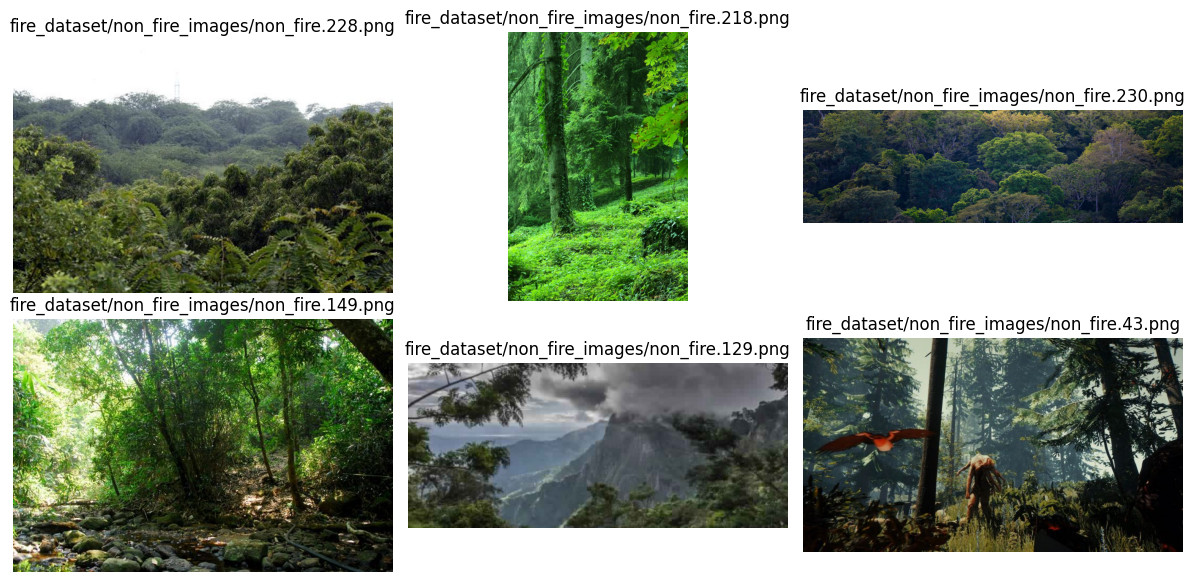
\includegraphics[width=0.90\textwidth]{images/Img_fire_label0_exp.png}
        \caption{Hình ảnh không lửa}
        \label{fig:Img_fire_label0_exp}
    \end{figure}
    \FloatBarrier

    \begin{figure}[htp]
        \centering
        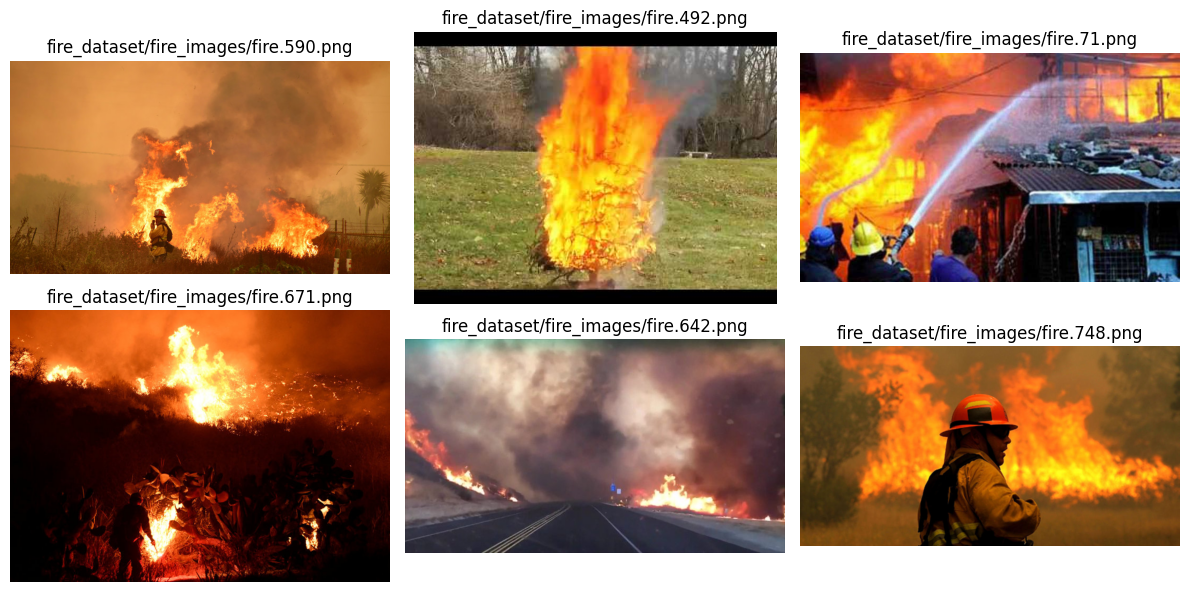
\includegraphics[width=0.90\textwidth]{images/Img_fire_label1_exp.png}
        \caption{Hình ảnh có đám cháy}
        \label{fig:Img_lung_label0_exp}
    \end{figure}
    \FloatBarrier

\subsubsection{Phân tích, trực quan hóa dữ liệu}

    \begin{figure}[htp]
        \centering
        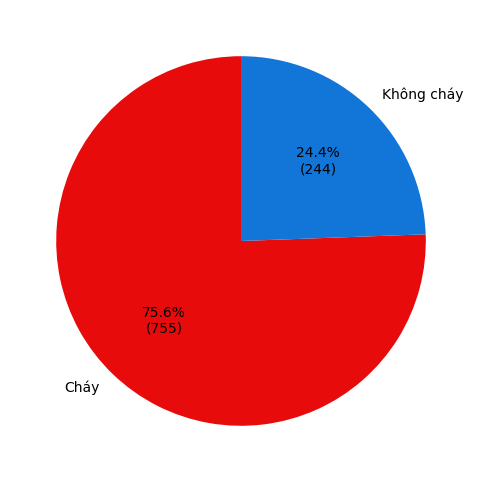
\includegraphics[width=0.50\textwidth]{images/Img_fire_label.png}
        \caption{Số lượng hình ảnh mỗi nhãn}
        \label{fig:Img_fire_label}
    \end{figure}
    \FloatBarrier

    Biểu đồ pie \ref{fig:Img_lung_label} cho thấy sự phân phối dữ liệu giữa hai nhãn. Ta thấy dữ liệu chứa nhiều hình ảnh có đám cháy hơn so với không, hình ảnh chứa đám cháy chiếm 75.6\% trong bộ dữ liệu

    \begin{figure}[htp]
        \centering
        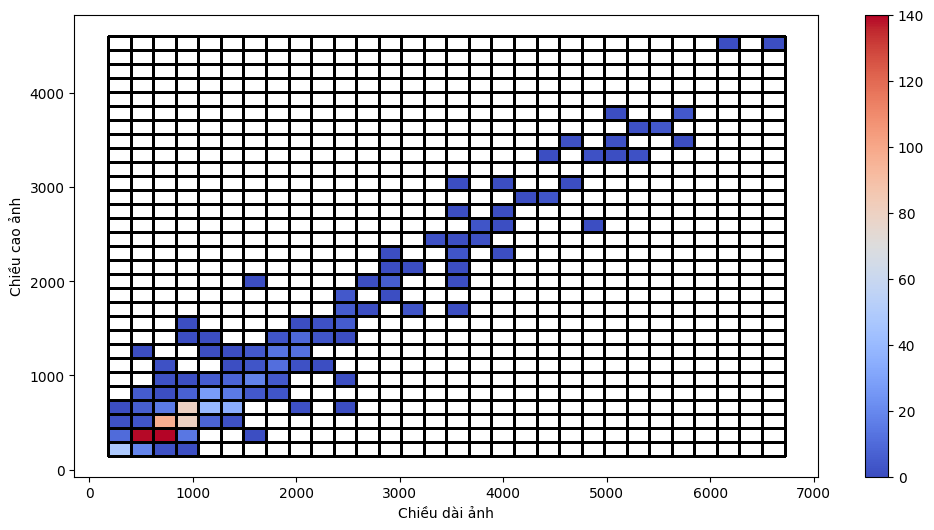
\includegraphics[width=0.90\textwidth]{images/Img_fire_resolution.png}
        \caption{Phân phối độ phân giải ảnh}
        \label{fig:Img_fire_resolution}
    \end{figure}
    \FloatBarrier

    Biểu đồ \ref{fig:Img_fire_resolution} thể hiện phân bố chiều dài và chiều cao ảnh của tập dữ liệu. Dễ thấy rằng phần lớn ảnh có kích thước phân giải nhỏ, kích thước phân giải càng lớn càng ít hình. Có một vài hình rất lớn.

    \begin{figure}[htp]
        \centering
        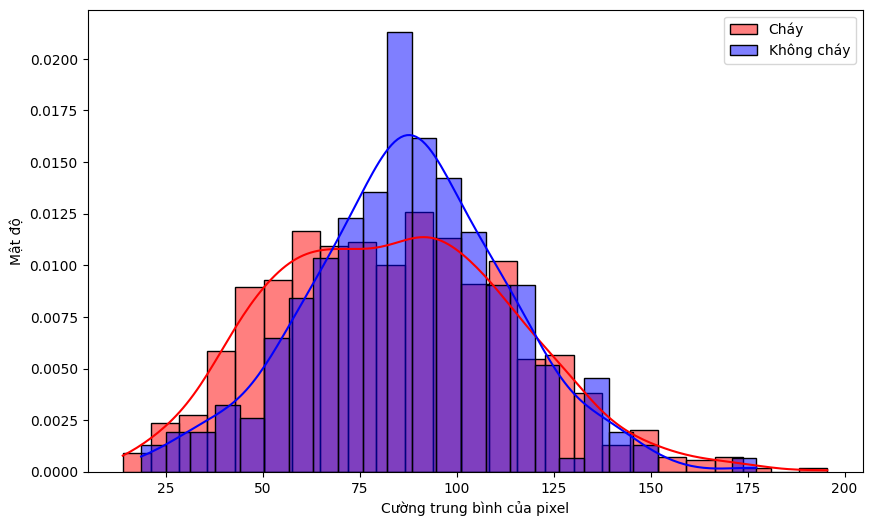
\includegraphics[width=0.90\textwidth]{images/Img_fire_gray_intensity.png}
        \caption{Phân phối cường độ trung bình ảnh}
        \label{fig:Img_fire_gray_intensity}
    \end{figure}
    \FloatBarrier

     Biểu đồ \ref{fig:Img_fire_gray_intensity} thể hiện sự phân phối cường độ pixel trung bình giữa hai nhóm ảnh. Cả hai phân phối đều có dáng hình chuông, tuy nhiên nhóm không cháy có đỉnh cao hơn và có dốc như phân phối chuẩn. Còn nhóm ảnh có đám cháy đỉnh thấp và trải rộng, cho thấy cường độ sáng thiếu đồng nhất, có thể là do sự xuất hiện của nguồn sáng (đám cháy) trong ảnh.

     \begin{figure}[htp]
        \centering
        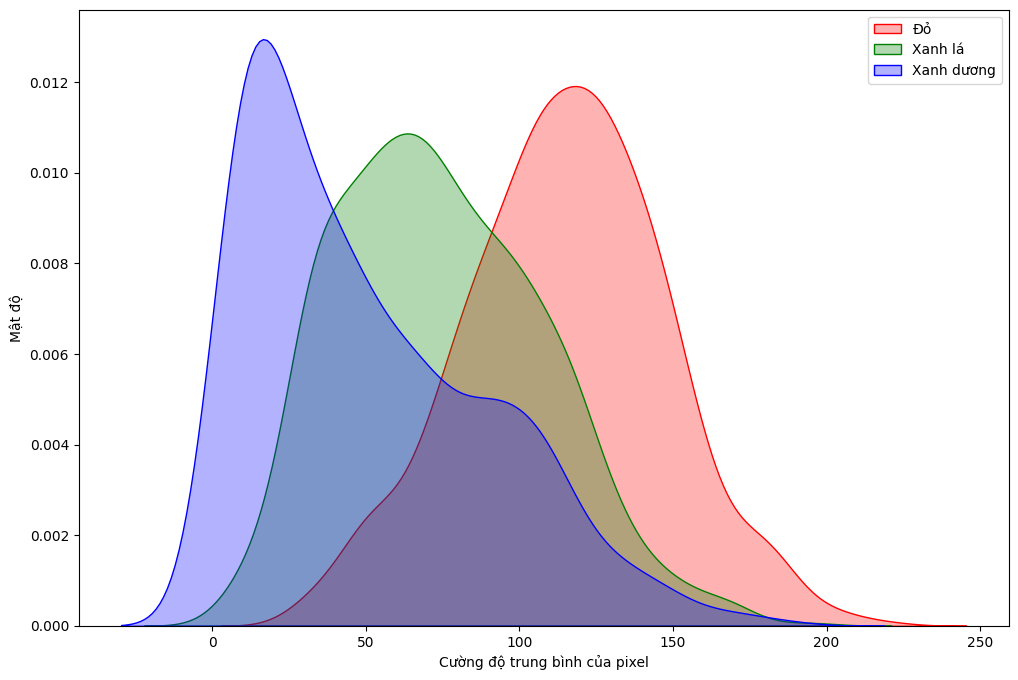
\includegraphics[width=0.90\textwidth]{images/Img_fire_rgb_intensity_fire.png}
        \caption{Phân phối cường độ trung bình các màu trong ảnh có đám cháy}
        \label{fig:Img_fire_rgb_intensity_fire}
    \end{figure}
    \FloatBarrier

    \begin{figure}[htp]
        \centering
        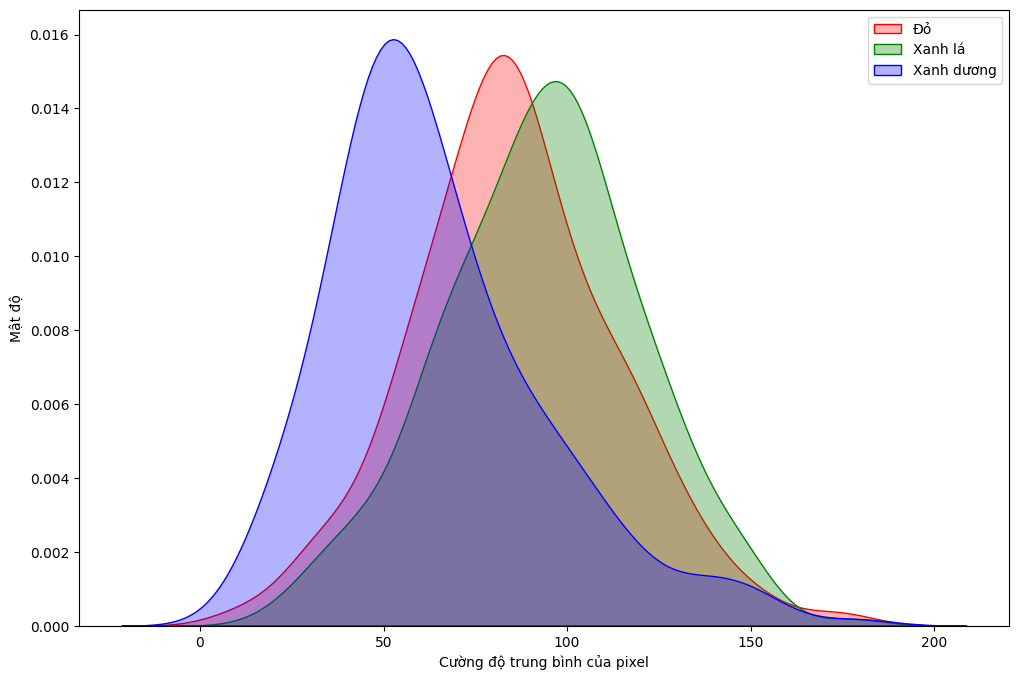
\includegraphics[width=0.90\textwidth]{images/Img_fire_rgb_intensity_nonfire.png}
        \caption{Phân phối cường độ trung bình các màu trong ảnh không có cháy}
        \label{fig:Img_fire_rgb_intensity_nonfire}
    \end{figure}
    \FloatBarrier

    Biểu đồ \ref{fig:Img_fire_rgb_intensity_fire} cho thấy kênh đỏ nổi bật hơn hẳn, với đỉnh phân bố cao và lệch phải, cho thấy cường độ đỏ trong các vùng cháy thường rất mạnh. Điều này phản ánh đặc tính quang phổ của lửa, vốn phát sáng chủ yếu trong vùng đỏ, cam. Kênh xanh dương lại có phân bố thấp và lệch trái rõ rệt, tập trung nhiều ở vùng cường độ thấp, cho thấy sự suy giảm đáng kể của màu xanh trong các khu vực bị ảnh hưởng bởi cháy, có thể do ánh sáng đỏ lấn át và khói làm tối các vùng ảnh. 

    Biểu đồ \ref{fig:Img_fire_rgb_intensity_nonfire} cho thấy trong ảnh không có cháy sự phân bố cường độ giữa ba kênh khá đồng đều và đối xứng, gần với phân phối chuẩn, thể hiện sự cân bằng tự nhiên của ánh sáng trong môi trường bình thường. Không có kênh màu nào quá trội, và ba đường phân bố chồng lấn nhau nhiều.

    \begin{figure}[htp]
        \centering
        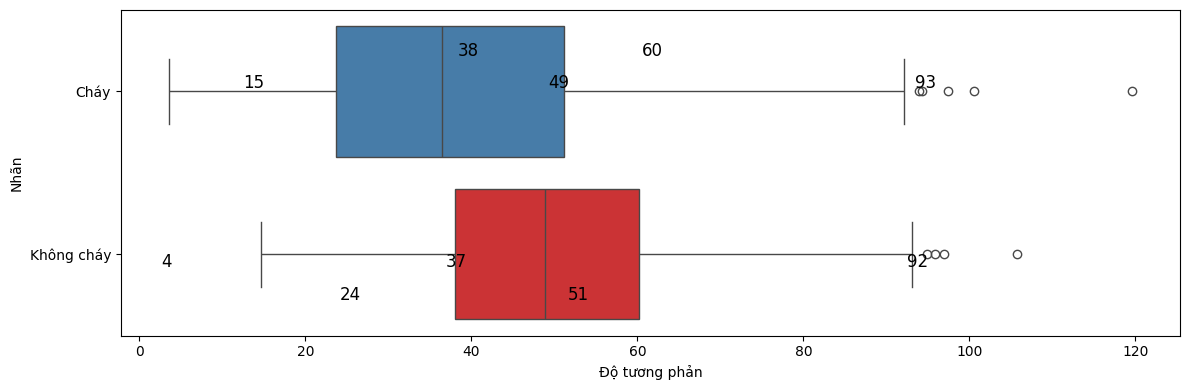
\includegraphics[width=0.90\textwidth]{images/Img_fire_rgb_blue_contrast.png}
        \caption{Độ tương phản kênh xanh dương theo nhãn}
        \label{fig:Img_fire_rgb_blue_contrast}
    \end{figure}
    \FloatBarrier

      Biểu đồ \ref{fig:Img_fire_rgb_blue_contrast} cho thấy rằng trong ảnh cháy, độ tương phản của kênh xanh dương có xu hướng thấp và ít biến động hơn, có thể do sự mất cân bằng màu khi ngọn lửa và khói làm giảm độ phân biệt sáng–tối ở vùng xanh dương. Trong khi đó, ở ảnh không cháy, kênh xanh dương giữ được sự phân tán rộng và mức độ tương phản cao hơn

    \begin{figure}[htp]
        \centering
        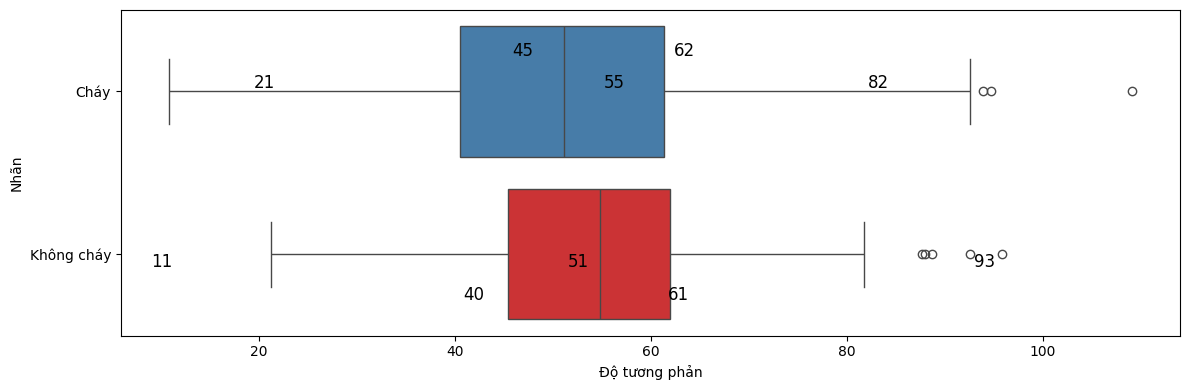
\includegraphics[width=0.90\textwidth]{images/Img_fire_rgb_green_contrast.png}
        \caption{Độ tương phản kênh xanh lá theo nhãn}
        \label{fig:Img_fire_rgb_green_contrast}
    \end{figure}
    \FloatBarrier

     Biểu đồ \ref{fig:Img_fire_rgb_green_contrast} cho thấy độ tương phản kênh xanh lá của hai loại hình ảnh khá tương đồng, với khá biệt duy nhất là khoảng tứ vị phân và hai đầu whisker của nhóm ảnh có đám cháy phân rộng hơn. 

    \begin{figure}[htp]
        \centering
        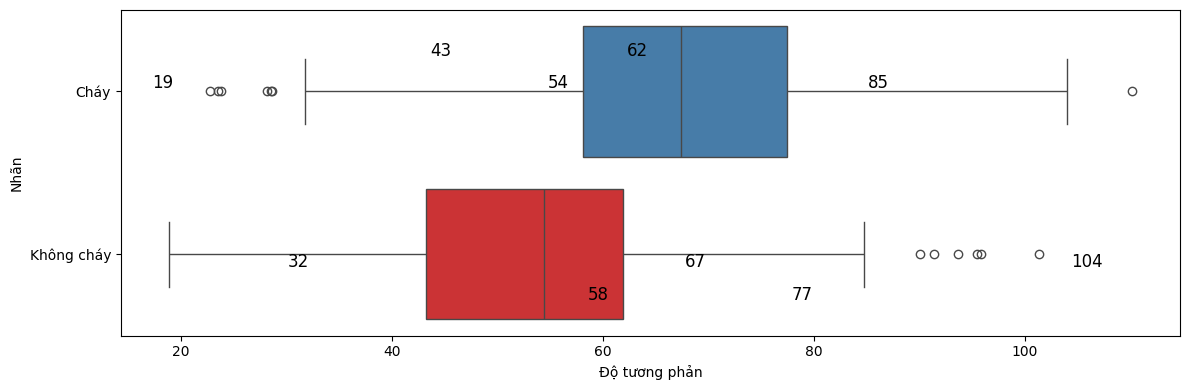
\includegraphics[width=0.90\textwidth]{images/Img_fire_rgb_red_contrast.png}
        \caption{Độ tương phản kênh đỏ theo nhãn}
        \label{fig:Img_fire_rgb_red_contrast}
    \end{figure}
    \FloatBarrier

    Biểu đồ \ref{fig:Img_fire_rgb_red_contrast} thể hiện rõ sự khác biệt về độ tương phản của kênh đỏ giữa hai nhóm ảnh cháy và không cháy. Ở ảnh cháy, độ tương phản tập trung nhiều hơn ở các giá trị cao, với phân bố nghiêng về phía phải và trung vị đạt mức 62, cho thấy lửa làm nổi bật các vùng màu đỏ. Ngược lại, ảnh không cháy có độ tương phản thấp hơn một chút, với trung vị 58 và phân bố hẹp hơn, tuy vẫn tồn tại một số ngoại lệ cao nhưng không đủ để đẩy toàn bộ phân bố lên. Sự khác biệt này cho thấy rằng trong điều kiện có cháy, vùng màu đỏ không chỉ trở nên sáng hơn mà còn có sự biến động cục bộ rõ rệt hơn, góp phần tạo ra tương phản cao và có thể dùng làm chỉ báo quan trọng trong việc nhận diện vùng cháy trong ảnh.


\subsubsection{Mô hình hóa dữ liệu}
    Để phục vụ bài toán phân loại ảnh, nhóm sử dụng đặc trưng màu được trích xuất bằng cách tính histogram màu ba chiều trong không gian RGB. Phương pháp này dựa trên việc đếm tần suất xuất hiện của các tổ hợp giá trị màu trong ảnh, sau khi phân chia từng kênh màu thành các khoảng giá trị rời rạc. Kết quả là một vector đặc trưng phản ánh phân bố tổng quát của màu sắc trong ảnh, được chuẩn hóa để đảm bảo khả năng so sánh giữa các mẫu và làm đầu vào cho mô hình học máy.

    \paragraph{Phân cụm sử dụng K-means}
    \leavevmode

    \begin{figure}[htp]
        \centering
        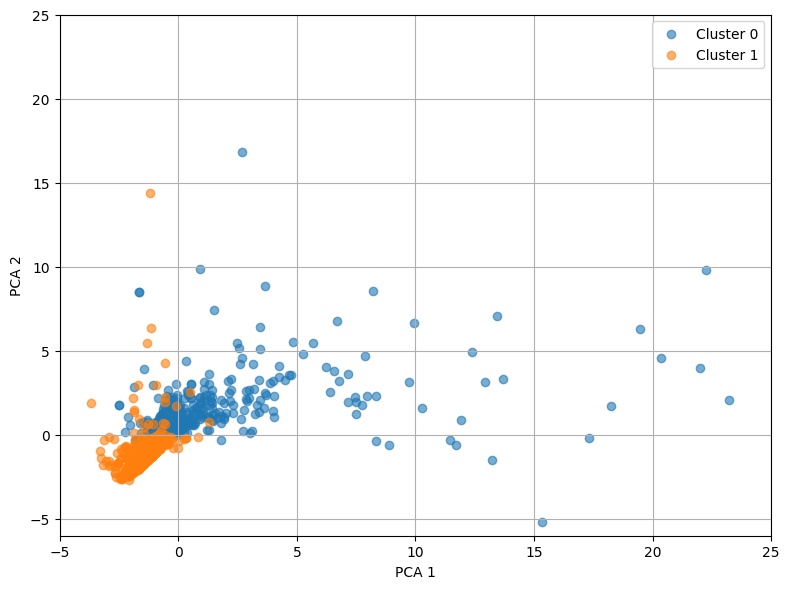
\includegraphics[width=0.90\textwidth]{images/Img_fire_kmeans.png}
        \caption{K-Means. ARI = 0.2899}
        \label{fig:Img_fire_kmeans}
    \end{figure}
    \FloatBarrier

    Biểu đồ \ref{fig:Img_fire_kmeans} thể hiện kết quả phân cụm ảnh K-Means trên dữ liệu ảnh đám cháy sau khi giảm chiều bằng PCA. Hai cụm không tách biệt rõ ràng. Các điểm dữ liệu của hai cụm có xu hướng chồng lấn lên nhau, đặc biệt tập trung gần gốc tọa độ. Chỉ số ARI đạt 0.2899, cho thấy mô hình phân cụm tương đối nhưng chưa sát với thực tế.
    

    \paragraph{Phân cụm sử dụng Spectral Clustering}
    \leavevmode

    \begin{figure}[htp]
        \centering
        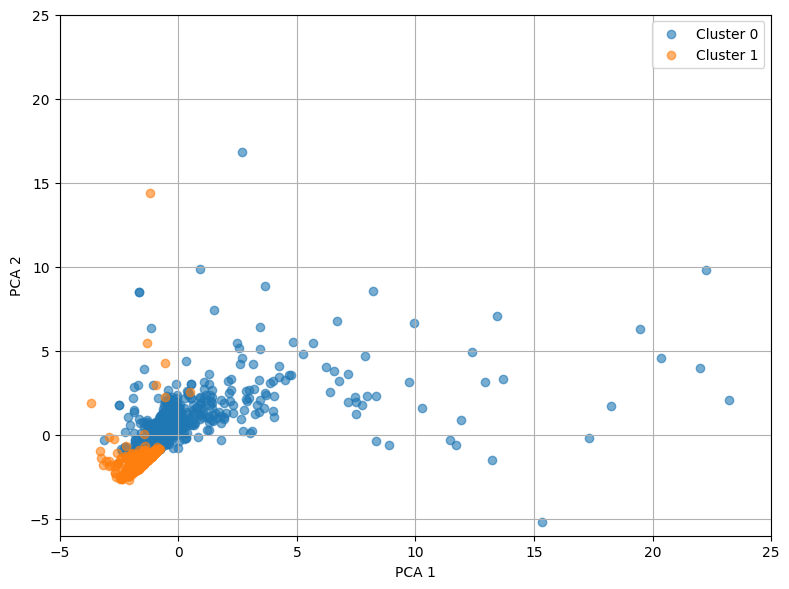
\includegraphics[width=0.90\textwidth]{images/Img_fire_spectral.png}
        \caption{Spectral Clustering. ARI = 0.0838}
        \label{fig:Img_fire_spectral}
    \end{figure}
    \FloatBarrier

    Biểu đồ \ref{fig:Img_fire_spectral} cho thấy kết quả phân cụm của thuật toán Spectral Clustering sau khi dữ liệu được giảm chiều bằng PCA. Các điểm dữ liệu của hai cụm chồng lấn nhiều. Giá trị ARI chỉ đạt 0.0838, cho thấy kết quả phân cụm gần như không tương quan với nhãn thực tế và hiệu quả phân cụm rất thấp.
    

    \paragraph{Phân cụm sử dụng Gaussian Mixture}
    \leavevmode
    
    \begin{figure}[htp]
        \centering
        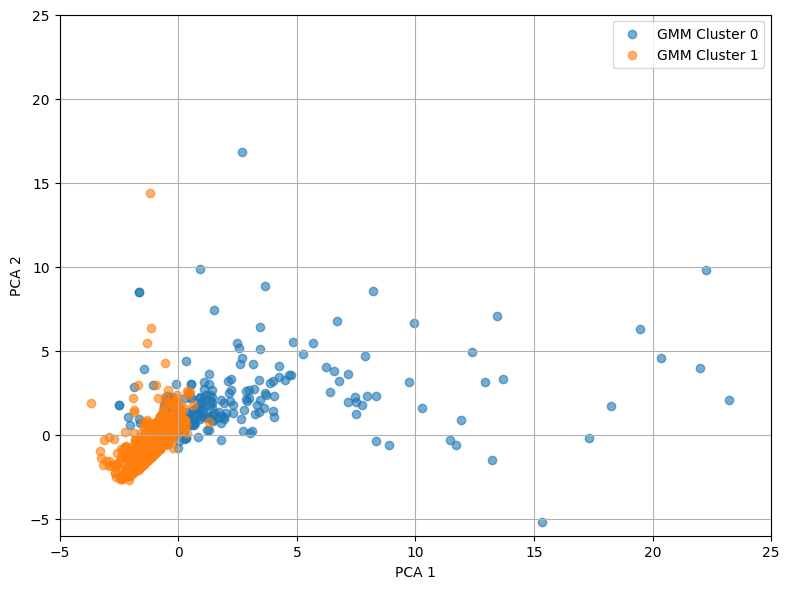
\includegraphics[width=0.90\textwidth]{images/Img_fire_gauss.png}
        \caption{Gaussian Mixture. ARI = 0.4966}
        \label{fig:Img_fire_gauss}
    \end{figure}
    \FloatBarrier

     Biểu đồ \ref{fig:Img_fire_gauss} cho thấy kết quả phân cụm của mô hình Gaussian Mixture sau khi dữ liệu được giảm chiều bằng PCA. Hai cụm được xác định rõ ràng, cụm màu cam tập trung chủ yếu ở vùng gần gốc tọa độ, trong khi cụm màu xanh lan rộng hơn phía ngoài phải. Mặc dù vẫn có một số điểm bị chồng lấn giữa hai cụm, nhưng sự tách biệt đã phần nào rõ ràng hơn. Chỉ số ARI đạt 0.4966, cao hơn đáng kể so với KMeans và Spectral Clustering, cho thấy GMM phản ánh cấu trúc dữ liệu tốt hơn và phân cụm có mức độ tương quan khá với nhãn thực tế.

    \begin{table}[htbp]
        \centering
        \caption{So sánh kết quả các mô hình}
        \label{tab:lung-clustering-compare}
        \begin{tabular}{|l|c|}
        \hline
        Model & ARI  \\
        \hline
        K-Means & 0.2899  \\
        \hline
        Spectral Clustering & 0.0838 \\
        \hline
        Gaussian Mixture & \textbf{0.4966}  \\
        \hline
        \end{tabular}
    \end{table}

    \FloatBarrier

    Bảng kết quả cho thấy mô hình Gaussian Mixture đạt hiệu suất cao nhất với chỉ số ARI là 0.4966, thể hiện khả năng phân cụm gần đúng với nhãn thực tế. K-Means đứng thứ hai với giá trị ARI 0.2899, cho thấy mức độ phân biệt cụm ở mức trung bình. Trong khi đó, Spectral Clustering có kết quả thấp nhất với ARI chỉ 0.0838, phản ánh khả năng phân cụm yếu và gần như không tương quan nhiều với cấu trúc thực tế của dữ liệu. Điều này cho thấy Gaussian Mixture là lựa chọn phù hợp hơn cả trong bài toán phân cụm này.